\section{Channel Capacity}

The `information' channel capacity of a DMC is defined as:
$$C\triangleq \max\limits_{p(x)}I(X;Y)$$
其中$p(y|x)$是已知的, $p(x)$是变量.

在第1章 Mutual Information中, 我们已经证明了 $H(X)$是关于$p(x)$的concave function, 由于
$$I(X;Y)=H(Y)-H(Y|X)=-\sum\limits_{y}p(y)\log p(y)-\sum_{x}p(x)H(Y|X=x)$$
其中$p(y)=\sum\limits_{x}p(x)p(y|x)$, 所以$p(y)$是$p(x)$的线性函数, 所以$I(X;Y)$是$p(x)$的concave function.

$I(X;Y)=f\left(p(x)\right)$ is a concave function of $p(x)$!

\begin{example}
Noisy channel with non-overlapping outputs. $C=1$ \textcolor{red}{bit per transmission}.
\begin{figure}[htbp]
    \centering
    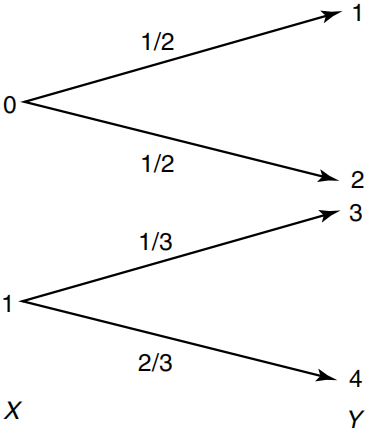
\includegraphics[width=0.3\textwidth]{./figures/chapter5/non_overlap.png}
\end{figure}
$$I(X;Y)=H(X)-H(Y|X)=H(X)\leq \log 2 =1$$
$$C=\max_{p(x)}I(X;Y)=1$$
When $p(x)=\left(\dfrac{1}{2},\dfrac{1}{2}\right)$, $C=1$ \textcolor{red}{bit per transmission}.

由$Y$可以直接得到$X$, 虽然由noisy, 但是noisy没有overlap, 不影响恢复出来$X$.
\end{example}

\begin{example}
Noisy typewriter.
\begin{figure}[htbp]
    \centering
    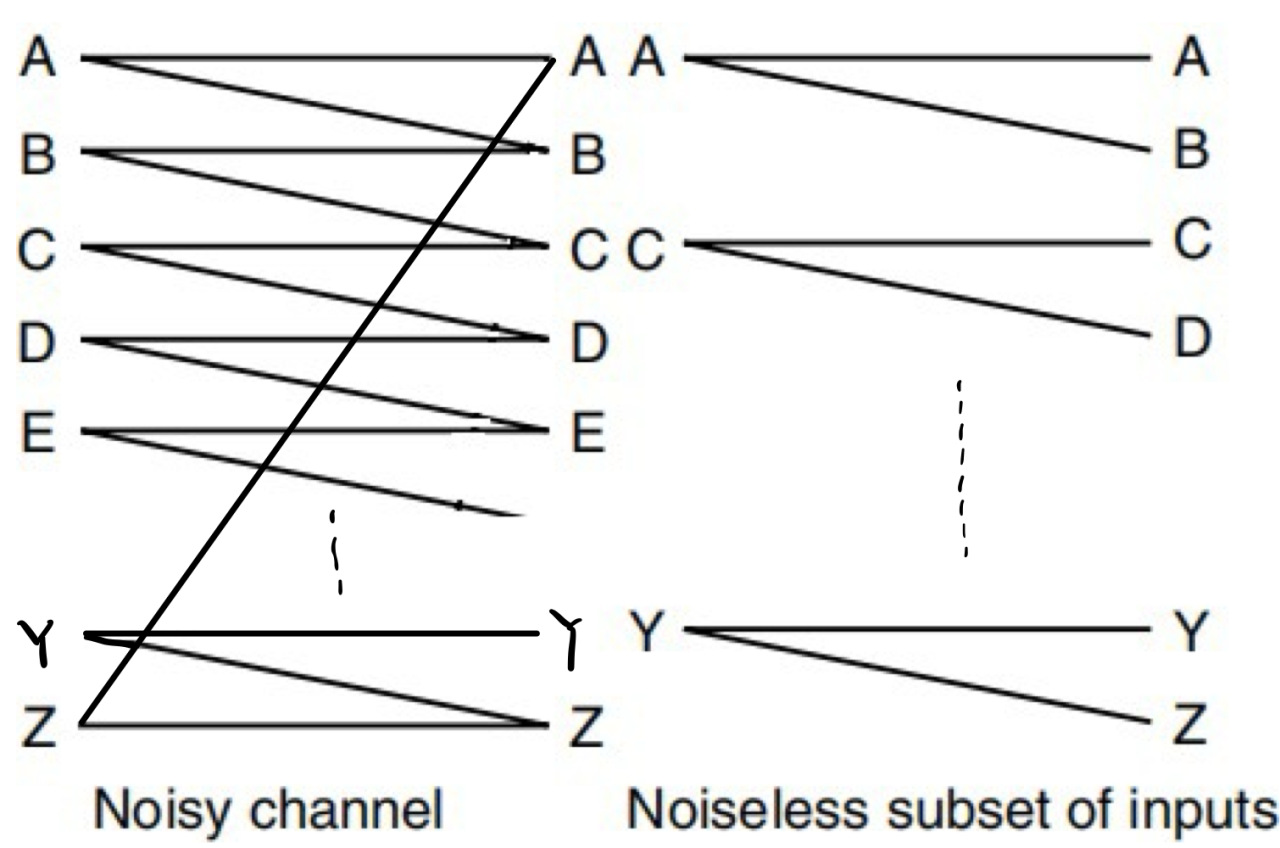
\includegraphics[width=0.5\textwidth]{./figures/chapter5/noisy_typewriter.png}
\end{figure}
$$I(X;Y)=H(Y)-H(Y|X)=H(Y)-H\left(\dfrac{1}{2},\dfrac{1}{2}\right)\leq \log 26 - \log 2 = \log 13$$
当$X\sim DUnif(26)$时, $Y\sim DUnif(26)$. 此时 $C$ 取到 $I(X;Y)$ 的最大值 $\log 13$ bits per transmission.
但是注意到, 若按上图右侧的选择方式(i.e. $P(X=`A')=P(X=`C')=\ldots=P(X=`Y')=\dfrac{1}{13},P(X=`B')=P(X=`D')=\ldots=P(X=`Z')=0$)仍能取到最大值.

可见达到信道容量的$p(X)$不唯一.
\end{example}

Noisy typewriter 平时出现的情况较少, 但BSC较为常见. e.g. 在硬盘读写时出现错误.

\begin{example}
Binary Symmetric Channel(BSC).
\begin{figure}[htbp]
    \centering
    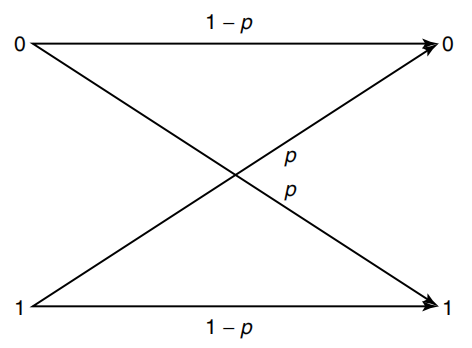
\includegraphics[width=0.5\textwidth]{./figures/chapter5/BSC.png}
\end{figure}
\begin{align*}
I(X;Y) &= H(Y)-H(Y|X) \\
&= H(Y) - \sum_{x}H(Y|X=x)p(X=x) \\
&= H(Y) - H\left(p, 1-p\right) \\
&\leq \log 2 - H\left(p, 1-p\right) \\
&= 1 - H\left(p, 1-p\right)
\end{align*}
When $p(X=0)=p(X=1)=\dfrac{1}{2}$, $P(Y=0)=P(Y=1)=\dfrac{1}{2}$, which makes the inequality take the equality.

So $C=\max\limits_{p(x)}I(X;Y)=1-H\left(p, 1-p\right)$.
\end{example}


\begin{example}
Binary Erasure Channel(BEC). 可以看作有$p$的概率丢包.
\begin{figure}[htbp]
    \centering
    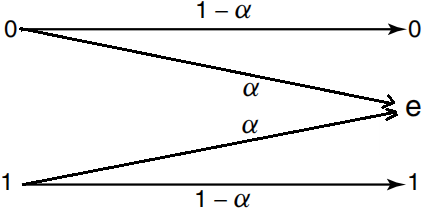
\includegraphics[width=0.5\textwidth]{./figures/chapter5/BEC.png}
\end{figure}

设$p(X=0)=\pi, p(X=1)=1-\pi$. 则
\begin{align*}
p(Y=e) &= \sum_xp(Y=e|X=x)p(X=x)=\alpha \\
p(X=0|Y=e) &= \dfrac{p(Y=e|X=0)p(X=0)}{p(Y=e)}=\pi
\end{align*}

<法一>.
\begin{align*}
    I(X;Y) &= H(X) - H(X|Y) \\
    &= H(X) - \sum_{y}H(X|Y=y)p(Y=y) \\
    &= H\left(\pi,1-\pi\right) - \alpha H\left(\pi,1-\pi\right) \\
    &= H\left(\pi,1-\pi\right)(1-\alpha) \\
    &\leq 1-\alpha
\end{align*}
当$p(x)=\left(\dfrac{1}{2},\dfrac{1}{2}\right)$时, $C=\max\limits_{p(x)}I(X;Y)=1-\alpha$.

<法二>. 设置辅助变量. $E$: indictor是否丢包.
$$E=\begin{cases}
    0, & \text{if } Y\neq e \\
    1, & \text{if } Y=e
\end{cases}$$
$$H(Y,E)=H(Y)+H(E|Y)=H(Y)$$
同时又有 $p(E=1)=p(Y=e)=\alpha$, 所以
\begin{align*}
H(Y,E) &= H(E)+H(Y|E)=H(\alpha)+(1-\alpha)H(\pi) \\
\Rightarrow \quad\ H(Y) &= H(\alpha)+(1-\alpha)H(\pi) \\
\Rightarrow \qquad\quad C &= H(Y) - H(Y|X) \\
&= H(\alpha)+(1-\alpha)H(\pi) - \pi H(\alpha) - (1-\pi)H(\alpha) \\
&= (1-\alpha)H(\pi) \\
&\leq 1-\alpha
\end{align*}
当$p(x)=\left(\dfrac{1}{2},\dfrac{1}{2}\right)$时, $C=\max\limits_{p(x)}I(X;Y)=1-\alpha$.

<法三>. $I(X;Y)=f(\pi)$是关于$\pi$的concave function. 一阶导数为0时取得最大值.
\end{example}


\begin{example}
Symmetric Channel. 若$p(y|x)$的转移矩阵满足: \\
1. 每一行都是其他行的置换(permutation). \\
2. 每一列都是其他列的置换(permutation). \\
则$C=\log\left|\mathcal{Y}\right|-H\left(\mathbf{r}\right)$. e.g. 图中例子 $C=\log 3-H\left(0.5,0.3,0.2\right)$.
\begin{figure}[htbp]
    \centering
    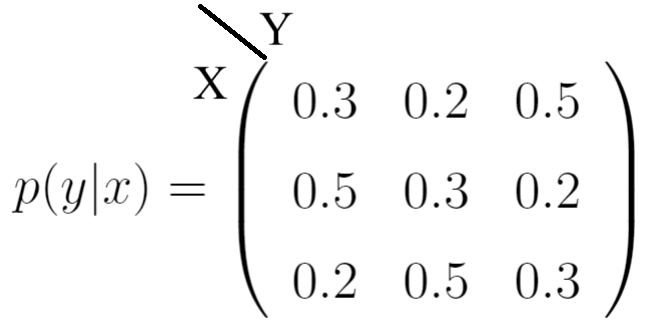
\includegraphics[width=0.5\textwidth]{./figures/chapter5/symmetric.png}
\end{figure}

Weak Symmetric Channel. 若$p(y|x)$的转移矩阵满足: \\
1. 每一行都是其他行的置换(permutation). \\
2. 每一列的和相等. \\
则$C=\log\left|\mathcal{Y}\right|-H\left(\mathbf{r}\right)$, $\mathbf{r}$是转移矩阵的行向量(都是相同行向量的置换).

Proof:
\begin{align*}
I(X;Y) &= H(Y)-H(Y|X) \\
&= H(Y)-\sum_{x}p(x)H(Y|X=x) \\
&= H(Y)-\sum_{x}p(x)H\left(\mathbf{r}\right) \\
&= H(Y)-H\left(\mathbf{r}\right) \\
&= \log\left|\mathcal{Y}\right|-H\left(\mathbf{r}\right)
\end{align*}
设每一列的和为同一个定值$\alpha$, 则当$p(x)=\dfrac{1}{\left|\mathcal{X}\right|}$时
$$p(Y=y)=\sum\limits_xp(Y=y|X=x)p(X=x)=\dfrac{\alpha}{\left|\mathcal{X}\right|}, \forall y\in\mathcal{Y}$$
所以所有的$y\in\mathcal{Y}$,概率相同. 即$p(Y=y)=\dfrac{1}{\left|\mathcal{Y}\right|}$. 此时取得$I(X;Y)$的最大值.
\end{example}


\begin{example}
Parallel Channel.
\begin{figure}[htbp]
    \centering
    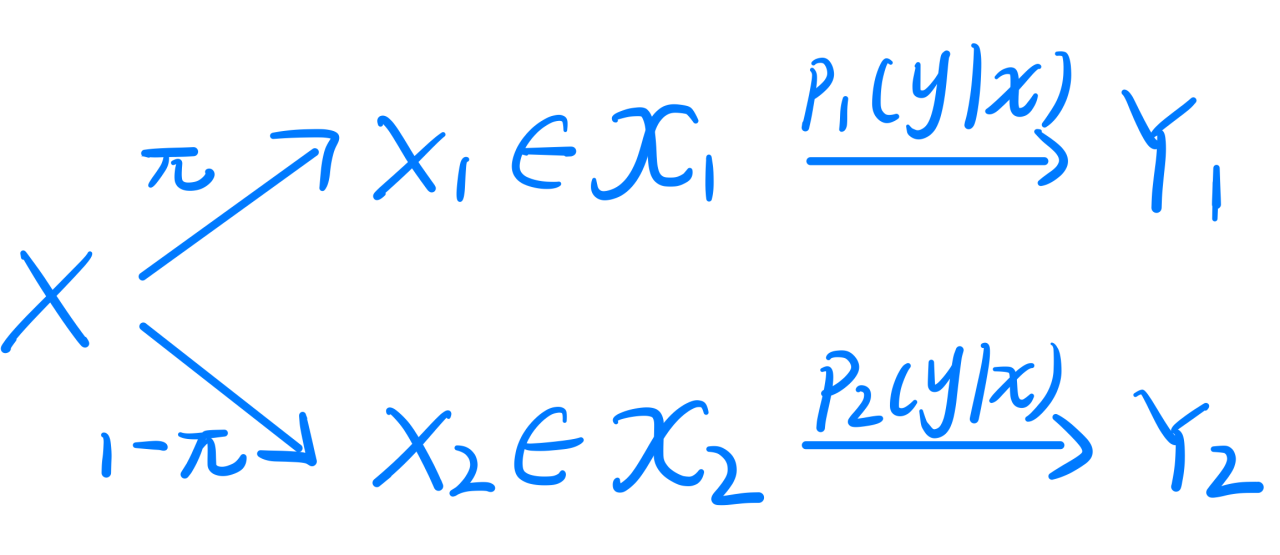
\includegraphics[width=0.45\textwidth]{./figures/chapter5/parallel.png}
\end{figure}

两个平行的信道容量分别为$C_1,C_2$, 则总容量满足
$$2^C=2^{C_1}+2^{C_2}$$
其中当$p(X\in\mathcal{X}_1)=\dfrac{2^{C_1}}{2^{C_1}+2^{C_2}}$, 且两个平行信道分别取得最大值时达到信道容量.

详见 Homework4 Problem 5.
\end{example}

In more general cases, 在开始时我们证明了 $I(X;Y)$是$p(x)$的concave function, 若没有闭式解, 我们可以用优化算法迭代求解.

通常采用 Frank-Wolfe grident search algorithm 或 Blahut-Arimoto算法求 $I(X;Y)$最大值. 详见 $\S 10.8$ (In book P358).

\begin{proposition}
Properties of channel capacity: \\
1. $C\geq 0 \qquad(I(X;Y)\geq 0)$ \\
2. $C\leq \log \left|\mathcal{X}\right|$, $C\leq \log \left|\mathcal{Y}\right|$.

Insight: 信道的input和output直接决定了capacity的上限, 可以看作输入和输出都会限制流量的宽度.

Proof: $I(X;Y)\leq \min\{H(X),H(Y)\} \leq \min\{\log\left|\mathcal{X}\right|,\log \left|\mathcal{Y}\right|\}$ \\
3. $I(X;Y)$是关于$p(x)$的concave function.
\end{proposition}